\documentclass[../main.tex]{subfiles}

\begin{document}
\chapter{Teoria degli anelli commutativi e dei campi}
\section{Insiemi}
Un insieme è una collezione di oggetti, detti elementi dell'insieme.
\begin{align*}
    \mathbb{N} & = \left\{ 0,1,2,3,\ldots \right\}                                        & \text{(Naturali)}  \\[1ex]
    \mathbb{Z} & = \left\{ \ldots,-2,-1,0,1,2,\ldots \right\}                             & \text{(Interi)}    \\[1ex]
    \mathbb{Q} & = \left\{ \frac{a}{b} \;\middle|\; a,b \in \mathbb{Z}, b \neq 0 \right\} & \text{(Razionali)} \\[1ex]
    \mathbb{R} & = \left\{ x \mid x \text{ è un numero reale }\right\}                    & \text{(Reali)}     \\[1ex]
    \mathbb{C} & = \left\{ a + bi \mid a,b \in \mathbb{R}, i^2=-1 \right\}                & \text{(Complessi)}
\end{align*}

\subsection{Operazioni tra insiemi}
\[
    \subseteq \;  \text{(Inclusione tra insiemi)} \qquad \subsetneq \; \text{(Inclusione propria tra insiemi)}
\]
\begin{note}
    $X \subseteq Y$ si legge $X$ è sottoinsieme di $Y$ o $X$ è incluso in $Y$.
\end{note}

\begin{definition}[Cardinalità]
    Se $X$ è un insieme finito, indico con $|X|$ il numero di elementi di $X$, detto anche la \textbf{cardinalità di $X$}.
\end{definition}

\begin{definition}[Insieme vuoto]
    L'insieme $\emptyset$ è l'insieme che non contiene alcun elemento. $\emptyset = \{ \}$ e $\abs{\emptyset} = 0$
\end{definition}

\begin{definition}[Prodotto Cartesiano]
    Siano $X$ e $Y$ due insiemi. L'insieme
    \[
        X \times Y := \{ (x,y) : x \in X , y \in Y \}
    \]
    è detto \textbf{prodotto cartesiano} di $X$ e $Y$.
\end{definition}

\begin{definition}[Insieme delle parti]
    \[
        \mathcal{P} (X) := \{ A : A \subseteq X \}
    \]
    è detto \textbf{Insieme delle parti di $X$}
\end{definition}

\begin{definition}[Complementare]
    Sia $A \in \mathcal{P} (x)$, l'insieme
    \[
        A^\mathrm{C} := \{ x \in X : x \notin A \}
    \]
    è detto \textbf{complementare} di $A$
\end{definition}

\section{Funzioni}
\begin{definition}[Funzione]
    Siano $X$ e $Y$ due insiemi. \textbf{Una funzione $f$ da $X$ a $Y$} è un sottoinsieme $F \subseteq X \times Y$ tale che:
    \begin{itemize}
        \item $(x, y_1) \in F$, $(x,y_2) \in F$ $\implies y_1 = y_2$, $\forall x \in X$, $y_1,y_2 \in Y$.
        \item $x \in X \implies \exists y \in Y \text{ tale che } (x,y) \in F$
    \end{itemize}
    Una funzione $F \subseteq X \times Y$ la indichiamo con $f : X \to Y$. E scriviamo $f(x) = y$ se $(x,y) \in F$.
\end{definition}

\begin{definition}[Funzione identità]
    La funzione $\Id_x : X \rightarrow X $ tale che
    \[
        \Id_x (x) = x, \forall x \in X
    \]
    è chiamata \textbf{funzione identità su $X$}.
\end{definition}

\begin{definition}[Funzione iniettiva]
    Una funzione $f: X \rightarrow Y$ è \textbf{iniettiva} se
    \[
        \forall x_1, x_2 \in X, f(x_1) = f(x_2) \implies x_1 = x_2
    \]

    ovvero se due elementi distinti di $X$ hanno immagini distinte.
\end{definition}

\begin{definition}[Funzione suriettiva]
    Una funzione $f: X \rightarrow Y$ è \textbf{suriettiva} se
    \[
        \Im(f) = Y
    \]
    dove
    \[
        \boxed{
            \Im(f) = \{ y \in Y : \exists x \in X : f(x) = y \}
        }
    \]
    è detta \textbf{immagine di $f$}.

    ovvero se ogni elemento di $Y$ è immagine di almeno un elemento di $X$, più elementi di $X$ possono avere la stessa immagine.
\end{definition}
\begin{note}[Diffrenza tra codominio e immagine]
    Il \textbf{codominio} di una funzione è l'insieme $Y$ mentre l'\textbf{immagine} è un sottoinsieme di $Y$ formato dagli elementi di $Y$ che sono effettivamente raggiungibili per qualche $x \in X$.
\end{note}

\begin{definition}[Preimmagine]
    Sia $f: X \rightarrow Y$ una funzione e $A \subseteq Y$. La \textbf{preimmagine di $A$} è l'insieme
    \[
        f^{-1}(A) := \{ x \in X : f(x) \in A \}
    \]
    Prendiamo quindi un sottoinsieme di $Y$ e guardiamo quali elementi di $X$ vengono mappati in $A$.
    \begin{note}
        E' la funzione inversa dell'immagine.
        \begin{itemize}
            \item $f^{-1}(\Im(f)) = f^{-1}(f(X)) = X$
        \end{itemize}
    \end{note}
\end{definition}

\begin{definition}[Funzione biunivoca]
    Una funzione $f: X \rightarrow Y$ è \textbf{biunivoca} se è sia iniettiva che suriettiva.

    Ovvero se ad ogni elemento di $X$ corrisponde un solo elemento di $Y$ e viceversa.
\end{definition}

\begin{figure}[h]
    \centering
    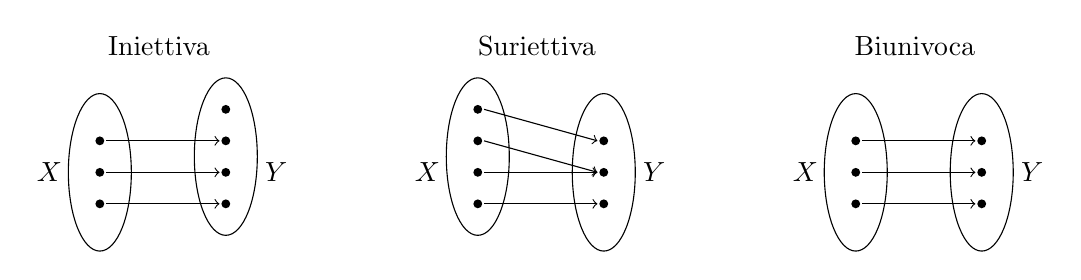
\begin{tikzpicture}[scale=0.8]
        % Injective function
        \begin{scope}[xshift=-6cm]
            \node[xshift=0.75cm] at (0,2) {Iniettiva};
            % Domain (X)
            \draw (0,0) ellipse (0.5cm and 1.25cm);
            \node at (-0.8,0) {$X$};
            \foreach \y in {-0.5,0,0.5} {
                    \fill (0,\y) circle (2pt);
                }
            % Codomain (Y)
            \draw (2,0.25) ellipse (0.5cm and 1.25cm);
            \node at (2.8,0) {$Y$};
            \foreach \y in {-0.5,0,0.5,1} {
                    \fill (2,\y) circle (2pt);
                }
            % Arrows
            \draw[->] (0.1,-0.5) -- (1.9,-0.5);
            \draw[->] (0.1,0) -- (1.9,0);
            \draw[->] (0.1,0.5) -- (1.9,0.5);
        \end{scope}

        % Surjective function
        \begin{scope}[xshift=0cm]
            \node[xshift=0.75cm] at (0,2) {Suriettiva};
            % Domain (X)
            \draw (0,0.25) ellipse (0.5cm and 1.25cm);
            \node at (-0.8,0) {$X$};
            \foreach \y in {-0.5,0,0.5,1} {
                    \fill (0,\y) circle (2pt);
                }
            % Codomain (Y)
            \draw (2,0) ellipse (0.5cm and 1.25cm);
            \node at (2.8,0) {$Y$};
            \foreach \y in {-0.5,0,0.5} {
                    \fill (2,\y) circle (2pt);
                }
            % Arrows
            \draw[->] (0.1,-0.5) -- (1.9,-0.5);
            \draw[->] (0.1,0) -- (1.9,0);
            \draw[->] (0.1,0.5) -- (1.9,0);
            \draw[->] (0.1,1) -- (1.9,0.5);
        \end{scope}

        % Bijective function
        \begin{scope}[xshift=6cm]
            \node[xshift=0.75cm] at (0,2) {Biunivoca};
            % Domain (X)
            \draw (0,0) ellipse (0.5cm and 1.25cm);
            \node at (-0.8,0) {$X$};
            \foreach \y in {-0.5,0,0.5} {
                    \fill (0,\y) circle (2pt);
                }
            % Codomain (Y)
            \draw (2,0) ellipse (0.5cm and 1.25cm);
            \node at (2.8,0) {$Y$};
            \foreach \y in {-0.5,0,0.5} {
                    \fill (2,\y) circle (2pt);
                }
            % Arrows
            \draw[->] (0.1,-0.5) -- (1.9,-0.5);
            \draw[->] (0.1,0) -- (1.9,0);
            \draw[->] (0.1,0.5) -- (1.9,0.5);
        \end{scope}
    \end{tikzpicture}
\end{figure}

\begin{definition}[Composizione di funzioni]
    Siano $f: X \rightarrow Y$ e $g: Y \rightarrow Z$ due funzioni. La \textbf{composizione di $f$ e $g$} è la funzione
    \[
        g \circ f : X \rightarrow Z \quad \text{t.c} \quad (g \circ f)(x) = g(f(x)), \forall x \in X
    \]
\end{definition}

\begin{definition}[Funzione invertibile]
    una funzione $f: X \rightarrow Y$ è detta \textbf{invertibile} se esiste una funzione $g: Y \rightarrow X$ tale che
    \begin{enumerate}[label=(\roman*)]
        \item $g \circ f = \Id_X$
        \item $f \circ g = \Id_Y$
    \end{enumerate}
    la funzione $g$ è detta \textbf{funzione inversa di $f$} e la indichiamo con $f^{-1}$.
\end{definition}
\begin{remark}
    Una funzione $f: X \rightarrow Y$ è invertibile se e solo se è \textbf{biunivoca}.
\end{remark}

\subsection{Operazioni su insiemi}

\begin{definition}[Operazione]
    Una funzione $f: X \times X \rightarrow X$ è detta \textbf{operazione su $X$}. Invece di $f(x,y)$
    scriveremo $x \cdot y$.
\end{definition}

\begin{definition}[Operazione associativa]
    Un'operazione $\cdot$ su $X$ è detta \textbf{associativa} se
    \[
        \boxed{
            (x \cdot y) \cdot z = x \cdot (y \cdot z) \qquad  \forall x,y,z \in X
        }
    \]
\end{definition}

\begin{definition}[Operazione commutativa]
    Un'operazione $\cdot$ su $X$ è detta \textbf{commutativa} se
    \[
        \boxed{
            x \cdot y = y \cdot x \qquad \forall x,y \in X
        }
    \]
\end{definition}

\begin{example}
    \
    \begin{itemize}
        \item $\mathcal{P}(X)$ con l'operazione di unione $\cup$ è associativa e commutativa, così come lo è con l'intersezione $\cap $.
        \item $A \setminus B  := A \cap B^C$ \textbf{(differenza insiemistica)} è un'operazione su $\mathcal{P}(X)$.

              Non è associativa: sia $A \neq \emptyset.$ Allora $A \setminus (A \setminus A) = A \neq (A\setminus A) \setminus A = \emptyset$

              Non è commutativa: $A \setminus \emptyset = A \neq \emptyset \setminus A = \emptyset$, se $A \neq \emptyset$
        \item $A \Delta B := (A \setminus B) \cup (B \setminus A)$ \textbf{(differenza simmetrica)}
              è un'operazione su $\mathcal{P}(X)$.

              è commutativa e anche associativa, facilmente verificabile coi diagrammi di Venn.
        \item Sia $F(X) := \{f : X\rightarrow X\}$.

              La composizione "$\circ$" è un'operazione su $F(X)$.

              è associativa, ma non è commutativa.
        \item $a \circ b = \frac{a + b}{2} $ è un'operazione commutativa su $\mathbb{Q}$, ma non associativa.
    \end{itemize}
\end{example}

\end{document}